\documentclass{beamer}
\usepackage{graphicx}
\usepackage{amsmath}
\usepackage{bibentry}


\graphicspath{{images/}}
\setbeamertemplate{footline}[frame number]
\setbeamertemplate{page number in head/foot}[appendixframenumber]
\usetheme{Darmstadt}

\title[short]{INTELLIGENT SYSTEMS}
\author[Flavio Forenza]{Flavio Forenza \\ \tiny flavio.forenza@studenti.unimi.it\\[5mm] 
\includegraphics[scale = 0.06]{logoUnimi2.png}}
\institute{Department of Computer Science,\\ University of Milan, Italy}
\date{\tiny \today}

\begin{document}

\begin{frame}
    \maketitle
\end{frame}


\logo{
\includegraphics[width=0.1\linewidth]{logoUnimi2.png}}
\section{Paper 1}
\subsection{\emph{"A Unified Framework for Salient StructureDetection by Contour-Guided Visual Search"}}
\begin{frame}
    \frametitle{INTRODUCTION}
    The purpose of the paper is to introduce a new method, in the 
    state of the art, which is able to identify regions and salient objects 
    within a scene simultaneously. The proposed system attempts to 
    bridge the gap between the two highly related tasks of \emph{"human 
    fixation"} prediction and \emph{"salient object detection"}, with a general 
    framework.
\end{frame}

\begin{frame}{RELATED WORK}
    To obtain the final result, two pathways are crossed (Fig.\ref{fid: flowchart}):
    \begin{enumerate}
        \item Selective
        \item Non-Selective
    \end{enumerate}
    \begin{figure}[htbp]
        \centering
        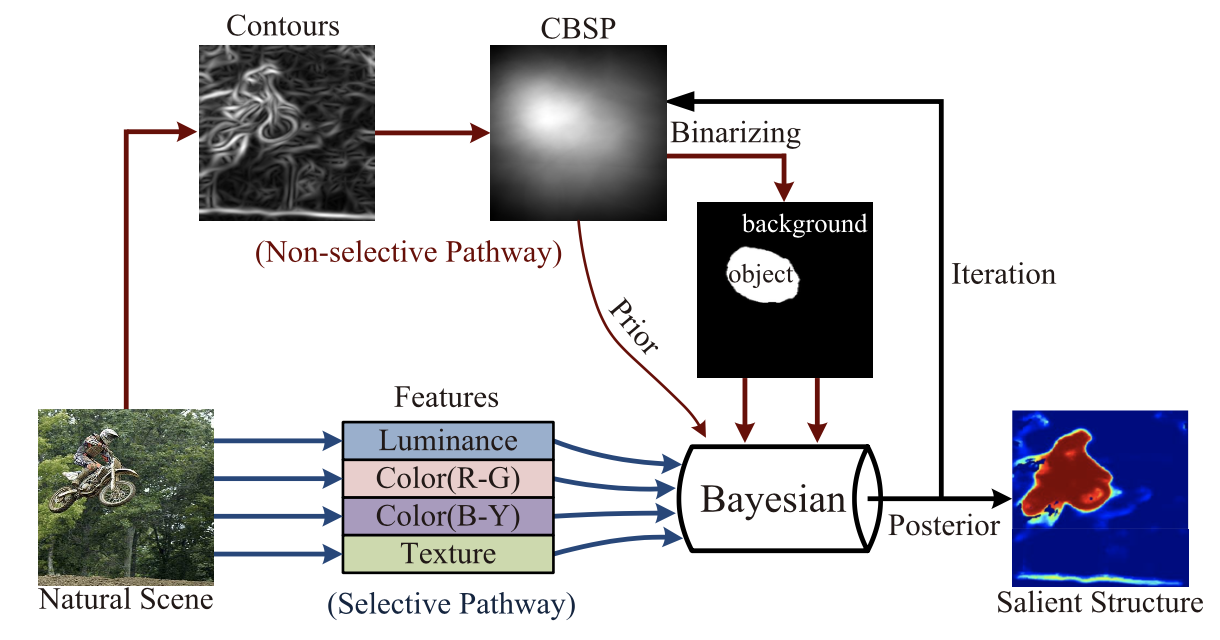
\includegraphics[width = 0.8\linewidth]{images/paper1/selective and non-selective pathways.png}
        \centering
        \caption{The flowchart of the porposed system.}
        \label{fid: flowchart}
    \end{figure}
\end{frame}

\begin{frame}{CONTOUR-GUIDED VISUAL SEARCH MODEL}
    In Non-Selective pathway are computed:
    \begin{enumerate}
        \item \emph{Contours} $\footnotemark $
        \item \emph{Contour-Based Spatial Prior} $ \rightarrow d_r = min (H, W) / 3$
    \end{enumerate}
    \bibliographystyle{abbrv}
    \bibliography{Bibliography}
    \footnotetext{\cite{0747815518}}
\end{frame}





    
\end{document}
